
\documentclass[nototal,handout]{beamer}
%\documentclass[nototal,handout]{beamer}

% This file is a solution template for:

% - Talk at a conference/colloquium.
% - Talk length is about 20min.
% - Style is ornate.


%
% In principle, this file can be redistributed and/or modified under
% the terms of the GNU Public License, version 2.
%
% However, this file is supposed to be a template to be modified
% for your own needs. For this reason, if you use this file as a
% template and not specifically distribute it as part of a another
% package/program, I grant the extra permission to freely copy and
% modify this file as you see fit and even to delete this copyright
% notice. 


\mode<presentation>
{
  \usetheme{Madrid}
  %\usetheme{Boadilla}
  % or ...

  \setbeamercovered{transparent}
  % or whatever (possibly just delete it)
}


\usepackage[english]{babel}
% or whatever

\usepackage[latin1]{inputenc}
% or whatever

\usepackage{times}
\usepackage[T1]{fontenc}
% Or whatever. Note that the encoding and the font should match. If T1
% does not look nice, try deleting the line with the fontenc.
\usepackage{graphicx} %sjr added
\graphicspath{{figures/}}
\usepackage{hyperref}
\author{\textsc{Sergio Rey}}
\institute[ASU]{\textbf{GPH 483/598}\\\textbf{Geographic Information
Analysis}\\School of Geographical Sciences\\Arizona State University\\Spring
2010}
\title[GPH 483/598]{Point Pattern Analysis: Processes}
\subtitle{}
\date[Point Pattern Processes]{}



% If you have a file called "university-logo-filename.xxx", where xxx
% is a graphic format that can be processed by latex or pdflatex,
% resp., then you can add a logo as follows:

% \pgfdeclareimage[height=0.5cm]{university-logo}{university-logo-filename}
% \logo{\pgfuseimage{university-logo}}



% Delete this, if you do not want the table of contents to pop up at
% the beginning of each subsection:
\AtBeginSubsection[]
{
  \begin{frame}<beamer>
    \frametitle{Outline}
    \tableofcontents[currentsection,currentsubsection]
  \end{frame}
}


% If you wish to uncover everything in a step-wise fashion, uncomment
% the following command: 

%\beamerdefaultoverlayspecification{<+->}


\begin{document}

\begin{frame}
  \titlepage
\end{frame}

\begin{frame}
  \frametitle{Outline}
  \tableofcontents
  % You might wish to add the option [pausesections]
\end{frame}


% Structuring a talk is a difficult task and the following structure
% may not be suitable. Here are some rules that apply for this
% solution: 

% - Exactly two or three sections (other than the summary).
% - At *most* three subsections per section.
% - Talk about 30s to 2min per frame. So there should be between about
%   15 and 30 frames, all told.

% - A conference audience is likely to know very little of what you
%   are going to talk about. So *simplify*!
% - In a 20min talk, getting the main ideas across is hard
%   enough. Leave out details, even if it means being less precise than
%   you think necessary.
% - If you omit details that are vital to the proof/implementation,
%   just say so once. Everybody will be happy with that.

\section{Properties of Point Processes}

\subsection{First Order Properties}
\begin{frame}[<+->]
  \frametitle{First Order Properties: Spatial Analysis}
  \begin{block}{Mean value of the process in space}
    \begin{itemize}
      \item Variation in mean value of the process in space
      \item Global, large scale spatial trend
    \end{itemize}
   \end{block}
   \begin{block}{First Order Property of Point Patterns, Intensity: $\lambda$}
     \begin{itemize}
      \item Intensity: $\lambda$ = number of events expected per unit area
       \item Estimation of $\lambda$
       \item Spatial variation of $\lambda$, $\lambda(s)$, $s$ is a location
     \end{itemize}
   \end{block}

   \begin{block}{}
     \begin{equation}
       \lambda(s) = \lim_{ds\rightarrow 0}\left\{ \frac{E(Y(ds))}{ds} \right\}
     \end{equation}
    \end{block}
 \end{frame}
\subsection{Second Order Property}
\begin{frame}[<+->]
  \frametitle{Second Order Properties: Spatial Analysis}
  \begin{block}{Spatial Correlation Structure}
    \begin{itemize}
      \item Deviations in values from process mean
      \item Local or small scale effects
    \end{itemize}
   \end{block}
   \begin{block}{Second Order Property of Point Patterns}
     \begin{itemize}
      \item Relationship between number of events in pairs of areas
       \item Second order intensity $\gamma(s_i,s_j)$
     \end{itemize}
   \end{block}

\begin{block}{}
     \begin{equation}
       \gamma(s_i,s_j) = \lim_{ds_i\rightarrow 0,ds_j\rightarrow 0}\left\{
       \frac{E(Y(ds_i)Y(ds_j))}{ds_ids_j} \right\}
     \end{equation}
    \end{block}

 \end{frame}

 \begin{frame}[<+->]
   \frametitle{Spatial Stationarity}
   \begin{block}{First Order Stationarity}
     \begin{equation}
       \lambda(s) = \lambda \forall s \in A
     \end{equation}
	\begin{equation}
	  E(Y(A)) = \lambda \times A
     \end{equation}
    \end{block}

    \begin{block}{Second Order Stationarity}
      \begin{equation}
	\gamma(s_i,s_j) = \gamma(s_i - s_j) = \gamma(h)
      \end{equation}
      \begin{itemize}
	\item $h$ is the vector difference between locations $s_i$ and $s_j$
	\item $h$ encompasses direction and distance (relative location)
	\item Second order intensity only depends on $h$ for second order stationarity
      \end{itemize}
    \end{block}
  \end{frame}

 \begin{frame}[<+->]
   \frametitle{Spatial Isotropy and Stationarity}
   \begin{block}{Isotropic Process}
     \begin{itemize}
       \item When a stationary process is invariant to rotation about the
	 origin.
       \item Relationship between two events depend only on the distance
	 separating their locations and not on their orientation to each
	 other.
       \item Depends only on distance, not direction
     \end{itemize}
    \end{block}

    \begin{block}{Usefulness}
      \begin{itemize}
	\item Two pairs of events from a stationary process
	  separated by same distance and relative direction should have same
	  ``relatedness''
	\item Two pairs of events from a stationary \emph{and} isotropic
	  process separated by the same distance (irrespective of direction)
	  should have the same ``relatedness''
	\item Both allow for replication and the ability to carry out
	  estimation of the underlying DGP.
      \end{itemize}
     \end{block}
  \end{frame}

  \section{Point Processes}
\subsection{Complete Spatial Randomness}
\begin{frame}
  \frametitle{Complete Spatial Randomness}
  \begin{block}{CSR}
    \begin{itemize}
      \item Standard of Reference
      \item Uniform: each location has equal probability
      \item Independent: location of points independent
      \item Homogeneous Planar Poisson Point Process
    \end{itemize}
   \end{block}
 \end{frame}




 \begin{frame}
   \frametitle{Poisson Point Process}
   \begin{block}{Intensity}
     \begin{itemize}
       \item number of points in region $A: N(A)$
       \item intensity: $\lambda = N/|A|$
       \item implies: $\lambda |A|$ points randomly scattered in a region with
	 area $|A|$
       \item e.g., $10\times 1$ (points per $km^2$)
     \end{itemize}
    \end{block}
    \begin{block}{Poisson Distribution}
      $N(A) \sim Poi(\lambda |A|)$
    \end{block}
  \end{frame}


  \begin{frame}
    \frametitle{Poisson Distribution}
    \begin{block}{Single Parameter Distribution: $\lambda |A|$}
      \begin{itemize}
	\item Generally, $\lambda$ is the number of events in some well
	  defined \emph{interval}
	  \begin{itemize}
	    \item Time: phone calls to operator in one hour
	    \item Time: accidents at an intersection per week
	     \item Space: trees in a quadrat
	  \end{itemize}
	\item Let $x$ be a Poisson random variable
	  \begin{itemize}
	    \item $E[x] = V[x]= \lambda |A|$
	  \end{itemize}
      \end{itemize}
     \end{block}
     \begin{block}{Poisson Distribution}
       \begin{equation}
	 P(x) =  \frac{e^{-\lambda |A|} (\lambda |A|)^x}{x!}
       \end{equation}
     \end{block}
   \end{frame}

   \begin{frame}
     \frametitle{Poisson Distribution $\lambda=2$}
     \begin{center}
       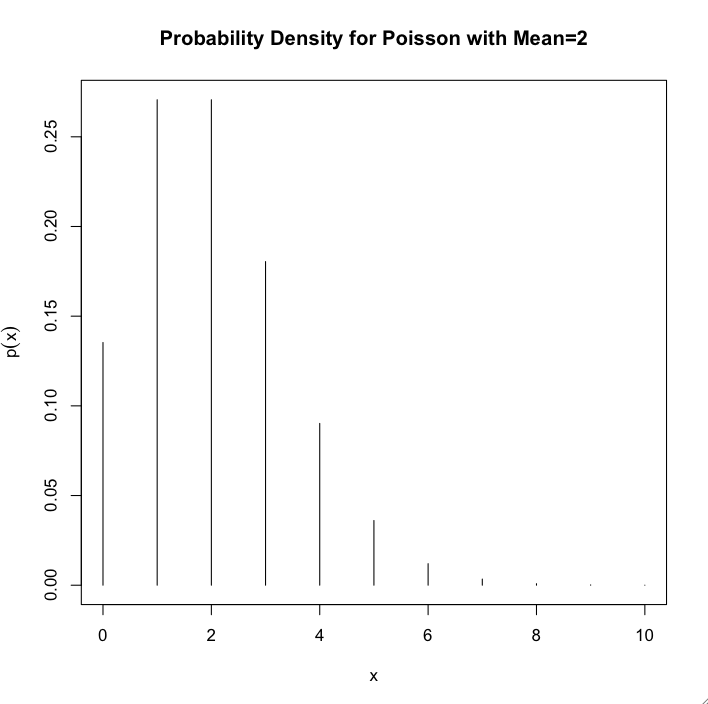
\includegraphics[width=.65\linewidth]{poisson2pdf.png}
     \end{center}
   \end{frame}


   \begin{frame}
     \frametitle{Poisson Distribution $\lambda=4$}
     \begin{center}
       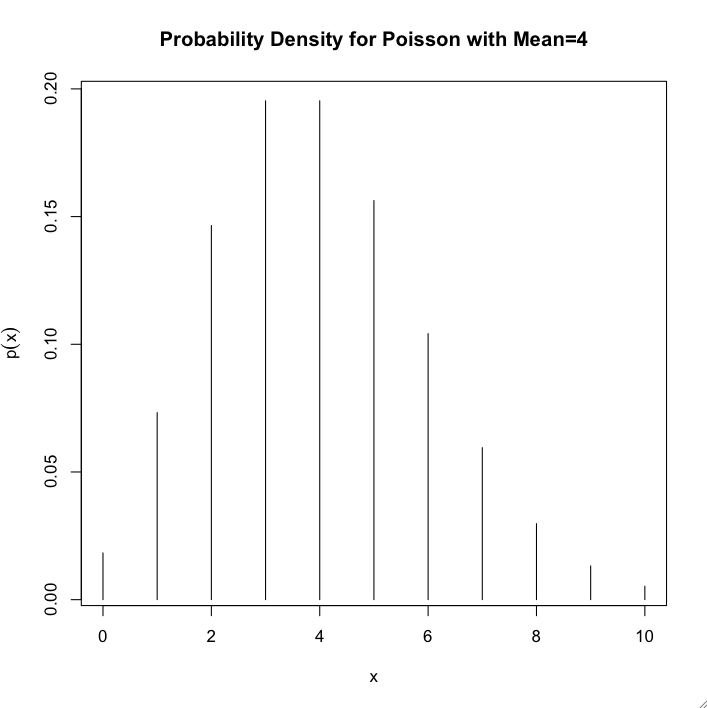
\includegraphics[width=.65\linewidth]{poisson4pdf.png}
     \end{center}
   \end{frame}

   \begin{frame}
     \frametitle{In Space}
     \begin{block}{Single Parameter}
      \begin{equation}
	P[N(A) = x ]= e^{-\lambda |A|} (\lambda |A|)^x /x!
      \end{equation}
      \end{block}
    \end{frame}

   \begin{frame}
     \frametitle{Spatial Example}
     \begin{block}{CSR with $\lambda = 5/km^2$}
       \begin{itemize}
	 \item Region = Circle
	   \begin{itemize}
	     \item area = $|A| = \pi r^2$
	     \item $r=0.1\ km$ then area $\approx 0.03 \ km^2$
	   \end{itemize}
	 \item Probability of Zero Points in Circle
	   \begin{eqnarray}
	     P[N(A) = 0] &= &  e^{-\lambda |A|} (\lambda |A|)^x /x!\\
	                 &\approx&e^{-5 \times 0.03} (5 \times 0.03)^0 /0!\\
	                 &\approx&e^{-5 \times 0.03} \\
	                 &\approx&0.86
	   \end{eqnarray}
       \end{itemize}
      \end{block}
    \end{frame}


 \begin{frame}[<+->]
   \frametitle{Complete Spatial Randomness (CSR)}
   \begin{block}{Homogeneous spatial Poisson point process}
     \begin{enumerate}
       \item The number of events occurring within a finite region $A$ is a
	 random variable following a Poisson distribution with mean
	 $\lambda|A|$, with $|A|$ denoting area of $A$.
       \item Given the total number of events $N$ occurring within an area $A$,
	 the locations of the $N$ events represent an independent random
	 sample of $N$ locations where each location is equally likely to be
	 chosen as an event.
     \end{enumerate}
   \end{block}
   \begin{block}{}
     \begin{itemize}
       \item Criterion 2 is the general concept of CSR (uniform (random))
	 distribution in $A$.
       \item Criterion 1 pertains to the intensity $\lambda$.
     \end{itemize}

    \end{block}

\end{frame}
\subsection{Homogeneous Poisson Process}
\begin{frame}[<+->]
  \frametitle{Homogeneous Poisson process}
  \begin{block}{Implications}
    \begin{enumerate}
      \item The number of events in nonoverlapping regions in $A$ are
	statistically independent.
      \item For any region $R \subset A$:
	\begin{equation}
	  \lim_{|R| \rightarrow 0} \frac{Pr[exactly\ one\ event\ in\ R]}{|R|}
	  = \lambda > 0
	\end{equation}
      \item \begin{equation}
	   \lim_{|R| \rightarrow 0} \frac{Pr[more\ than\ one\ event\ in\
	   R]}{|R|} = 0
	\end{equation}
    \end{enumerate}
   \end{block}
 \end{frame}

\begin{frame}[<+->]
  \frametitle{Homogeneous Poisson process}
  \begin{block}{Implications}
    \begin{itemize}
      \item $\lambda$ is the intensity of the spatial point pattern.
      \item For a Poisson random variable, $Y$:
	\begin{equation}
	  E[Y] = \lambda = V[Y]
	\end{equation}
      \item Provides the motivation for some quadrat tests of CSR hypothesis. 
	\begin{itemize}
	  \item If $Y_R$ is the count in quadrat $R$
	  \item If $\widehat{E[Y]}< \widehat{V[Y]}$: overdispersion = spatial clustering
	  \item If $\widehat{E[Y]}> \widehat{V[Y]}$: underdispersion = spatial uniformity
	\end{itemize}
    \end{itemize}
   \end{block}
 \end{frame}

 \begin{frame}
   \frametitle{Simulating CSR}
   \begin{block}{$N-conditioned$}
     \begin{itemize}
       \item CSR= uniform distribution
       \item random uniform draws for $x$ and $y$ point coordinates
       \item $N$ fixed
     \end{itemize}
    \end{block}
\begin{block}{$\lambda-conditioned$}
     \begin{itemize}
       \item CSR= Poisson distribution
       \item $\lambda$ and $|A|$ given
       \item $N(A)$ random
     \end{itemize}
    \end{block}
  \end{frame}


\begin{frame}
	\frametitle{CSR Uniform}
 \begin{figure}[ht]
  \begin{minipage}[b]{0.4\linewidth}
  \centering
  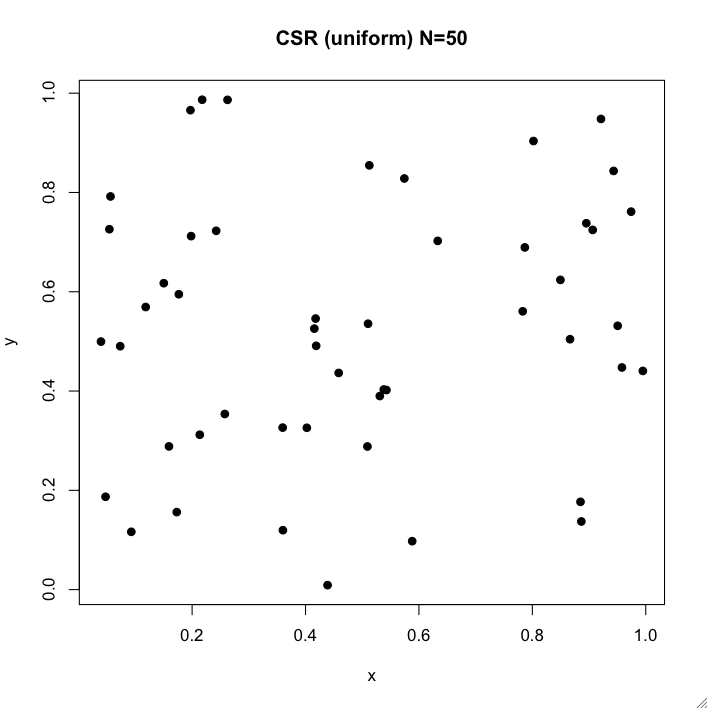
\includegraphics[scale=0.20]{csru50.png}
  \end{minipage}
  \begin{minipage}[b]{0.4\linewidth}
  \centering
  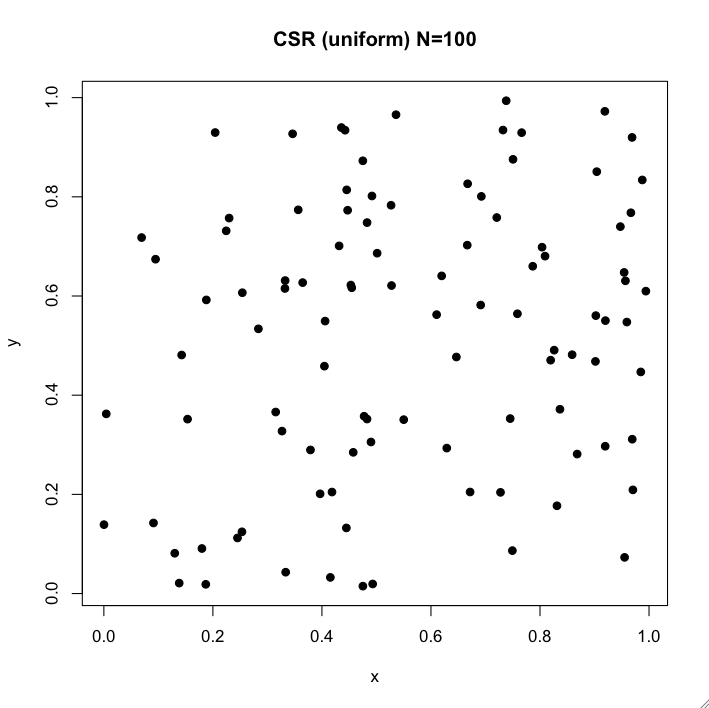
\includegraphics[scale=0.20]{csru100.png}
  \end{minipage}

  \end{figure}
 \end{frame} 


\begin{frame}
	\frametitle{CSR Poisson}
 \begin{figure}[ht]
 \begin{minipage}[b]{0.4\linewidth}
  \centering
  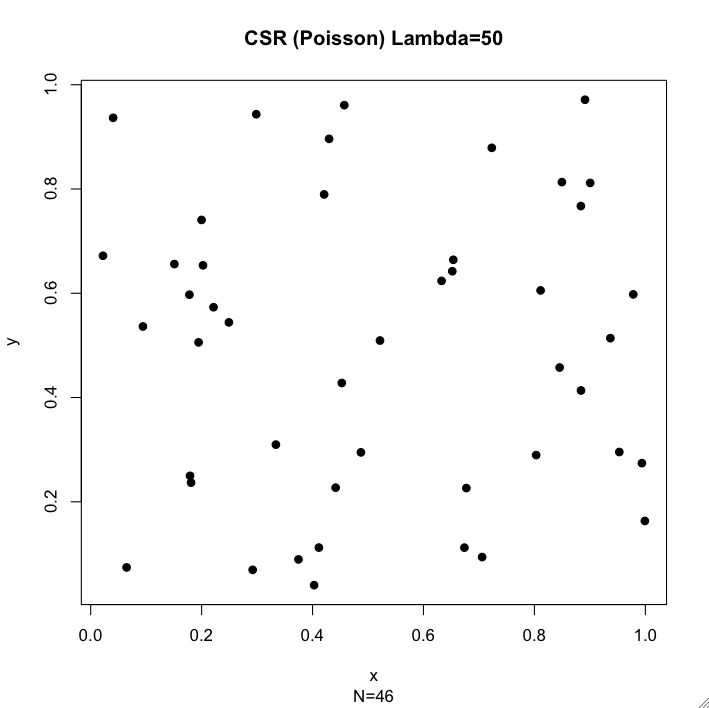
\includegraphics[scale=0.20]{csrp50.png}
  \end{minipage}
 \begin{minipage}[b]{0.4\linewidth}
  \centering
  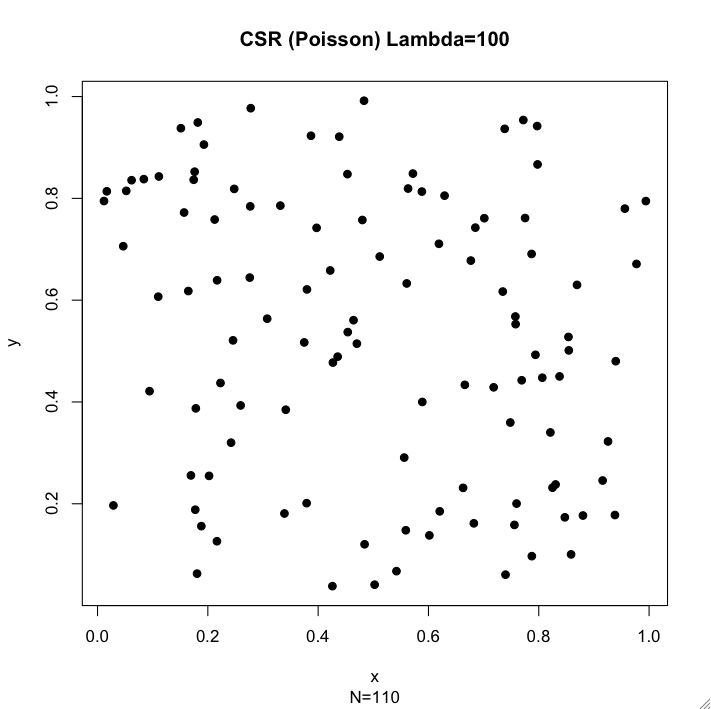
\includegraphics[scale=0.20]{csrp100.png}
  \end{minipage}
  \end{figure}
 \end{frame} 


  \begin{frame}
    \frametitle{Limitations of CSR}
    \begin{block}{Stationary Poisson Process}
      \begin{itemize}
	\item homogeneous
	\item translation invariant
      \end{itemize}
     \end{block}
     \begin{block}{Rare in practice}
       very few (any?) actual processes are CSR
      \end{block}
     \begin{block}{Strawman}
       \begin{itemize}
	 \item purely a benchmark
	 \item null hypothesis
       \end{itemize}
      \end{block}
   \end{frame}
   \subsection{Inhomogeneous Poisson Process (IPP)}
 \begin{frame}[<+->]
   \frametitle{Inhomogeneous Poisson Process (IPP)}
   \begin{block}{Criteria}
     \begin{enumerate}
       \item The number of events occurring within a finite  region $A$ is a
	 random variable following a Poisson Distribution with mean
	 $\int_{A}\lambda(s) ds$.
       \item Given the total number of events $N$ occurring within $A$, the
	 $N$ events represent an independent sample of $N$ locations, with the
	 probability of sampling a particular point $s$ proportional to
	 $\lambda(s)$.
     \end{enumerate}
    \end{block}
    \begin{block}{Spatially Variable Intensity $\lambda(s)$}
      \begin{itemize}
	\item Useful for \emph{constant risk hypothesis}
	\item Underlying population at risk is spatially clustered
	\item Want to control for that since with individual constant risk
	  apparent clusters would be generated.
	\item Compare pattern against constant risk, not CSR.
      \end{itemize}
    \end{block}
  \end{frame}

\begin{frame}[<+->]
  \frametitle{Inhomogeneous Poisson Process}
  \begin{block}{Implications}
    \begin{itemize}
      \item Apparent clusters can occur solely due to heterogeneities in the intensity
	function $\lambda(s)$.
      \item Individual event locations still remain independent of one
	another.
      \item Process is not stationary due to intensity heterogeneity
    \end{itemize}
   \end{block}
   \begin{block}{HPP vs. IPP}
       HPP is a special case of IPP with a constant intensity
   \end{block}
 \end{frame}

\begin{frame}[<+->]
  \frametitle{CSR vs. Constant Risk Hypotheses}
  \begin{block}{CSR}
    \begin{itemize}
      \item Intensity is spatially constant 
      \item Population at risk assumed spatially uniform 
      \item Useful null hypothesis if these conditions are met
    \end{itemize}
   \end{block}
  \begin{block}{Constant Risk Hypothesis}

    \begin{itemize}
      \item Population density variable
      \item Individual risk constant
      \item Expected number of events should vary with population density
      \item Clusters due to deviation from CSR
      \item Clusters due to deviation from CSR and Constant Risk
    \end{itemize}

  \end{block}
 \end{frame}

\end{document}
